\begin{frame}
{Digital set peculiarities}

\textbf{Exact sampling x digitization}

\begin{center}
\begin{tabular}{ccc}
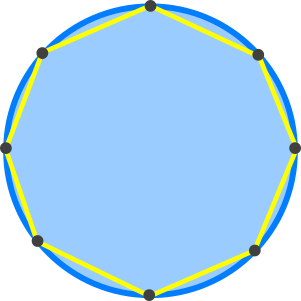
\includegraphics[scale=0.45]{figures/digital-estimators/exact-sampling/sampling-0.png}&
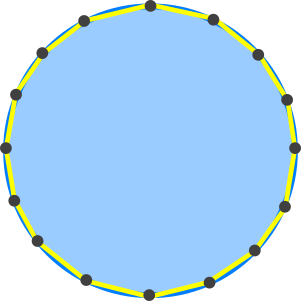
\includegraphics[scale=0.45]{figures/digital-estimators/exact-sampling/sampling-1.png}&
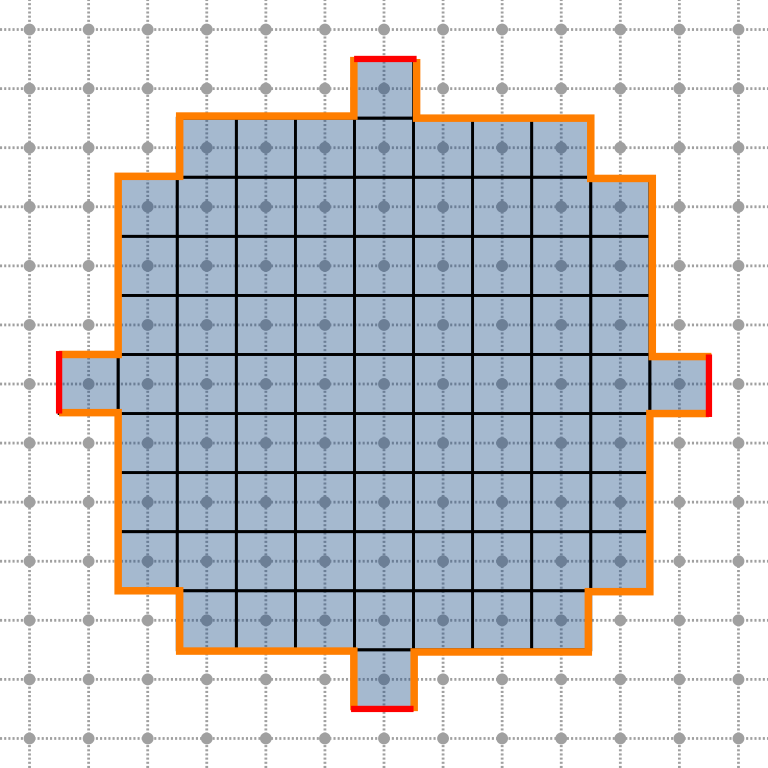
\includegraphics[scale=0.22]{figures/digital-estimators/exact-sampling/digital-ball-perimeter.png}
\end{tabular}
\end{center}

\pause
\textbf{Digitization ambiguity}

\begin{center}
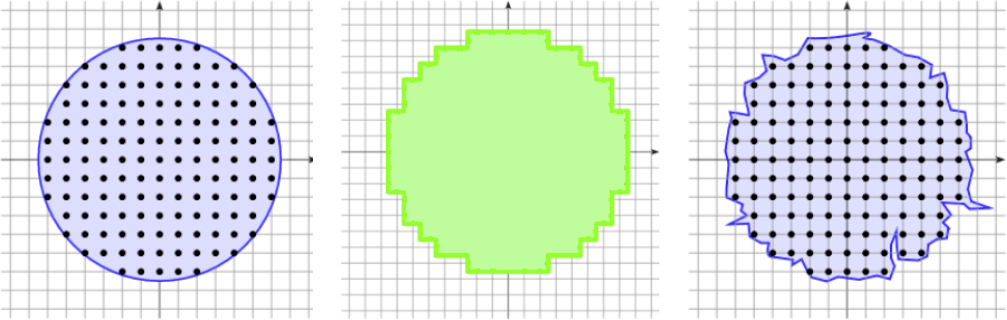
\includegraphics[scale=1]{figures/digital-estimators/exact-sampling/ambiguity.png}
\end{center}

\end{frame}

\begin{frame}
{Multigrid convergent estimators}

\footnotesize

\center
Disk of radius $5 (Area\approx78.54).$ 

\center
\begin{tabular}{ccc}
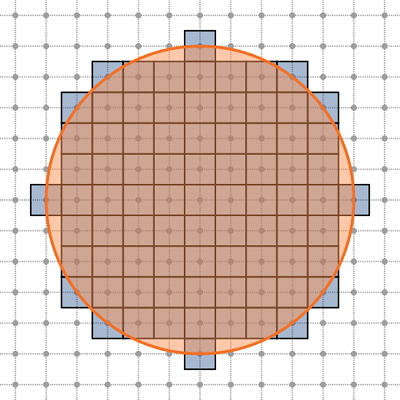
\includegraphics[scale=0.4]{figures/digital-estimators/multigrid/h1.png} &
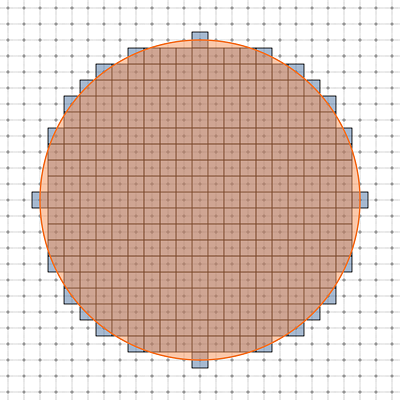
\includegraphics[scale=0.4]{figures/digital-estimators/multigrid/h05.png} &
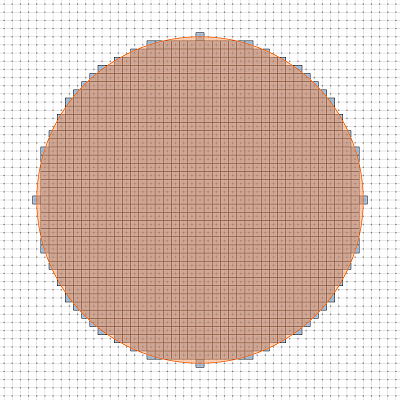
\includegraphics[scale=0.4]{figures/digital-estimators/multigrid/h025.png} \\
$h=1.0,\; \widehat{A}=81.$ & $h=\frac{1}{2},\; \hat{A}=79.25.$ & $h=\frac{1}{4},\; \hat{A}=78.56.$\\[1em]

\includegraphics[scale=0.4]{figures/digital-estimators/multigrid/h00625.png} &

\includegraphics[scale=0.4]{figures/digital-estimators/multigrid/h003125.png} &

\includegraphics[scale=0.4]{figures/digital-estimators/multigrid/h003125.png} \\
$h=\frac{1}{16},\; \hat{A}=78.44.$ & $h=\frac{1}{32},\; \hat{A}=78.5.$ & $h=\frac{1}{64},\; \hat{A}=78.53.$
\end{tabular}

\end{frame}

\begin{frame}
	{Digital sets and convergent estimators}	
	{Multigrid convergent estimators}	
%
	\begin{itemize}
		\onslide<1->{\item{Minimum Length Polygon (MLP)~\mycite{sloboda98approximation}}
		\begin{itemize}
			\item{Proved multigrid convergent for piecewise $3$-smooth convex shapes.}
		\end{itemize}}
		\onslide<3->{\vspace{2em}
		\item{Integral Invariant (II)~\mycite{coeurjolly13integral}}
		\begin{itemize}
			\item{Proved multigrid convergent for $C^2$ convex shapes with bounded curvature.}
		\end{itemize}}		
	\end{itemize}
	
	\onslide<2>{
	\begin{figure}
	\begin{tikzpicture}[overlay, remember picture] 
	\node at (current page.center) 
	    [
	    anchor=center,
	    xshift=0mm,
	    yshift=0mm
	    ] 
	{
	
	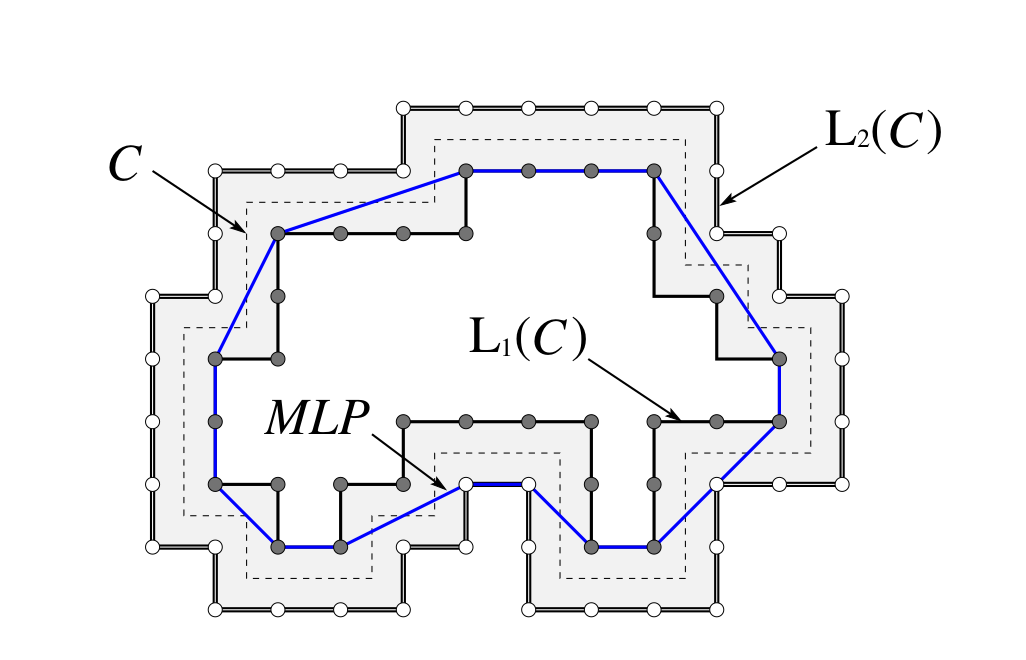
\includegraphics[scale=1.0]{figures/digital-estimators/mlp.png}
		
	};
	\end{tikzpicture}	
	\end{figure}	
	}
	
	\onslide<4->{
	\begin{figure}
	\begin{tikzpicture}[overlay, remember picture] 
	\node at (current page.center) 
	    [
	    anchor=center,
	    xshift=0mm,
	    yshift=0mm
	    ] 
	{
	\only<4>{
	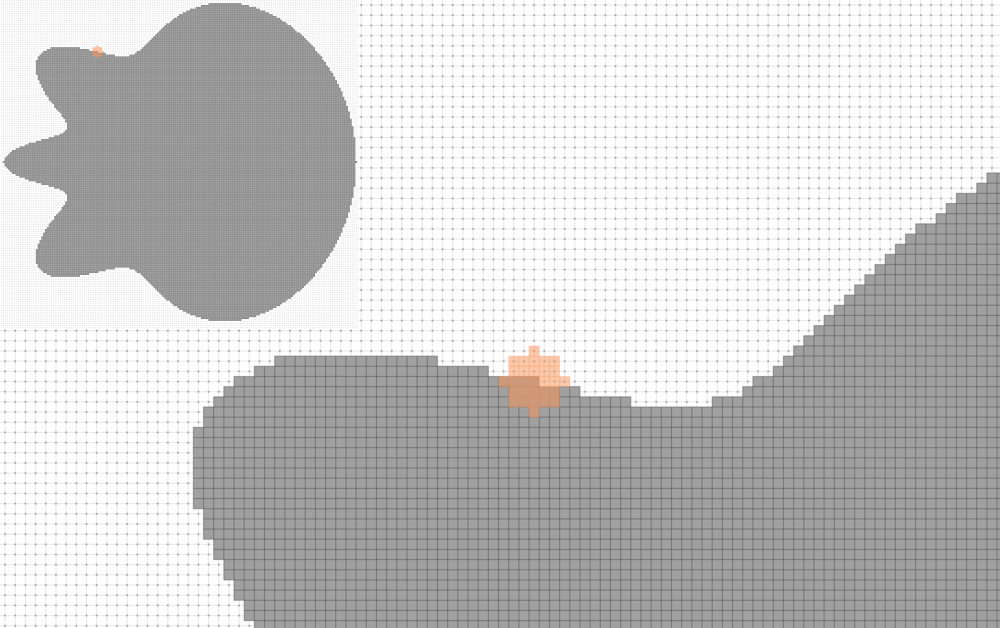
\includegraphics[scale=0.5]{figures/digital-estimators/ii/zoom/fr3-zoom.png}}%
	\only<5>{
	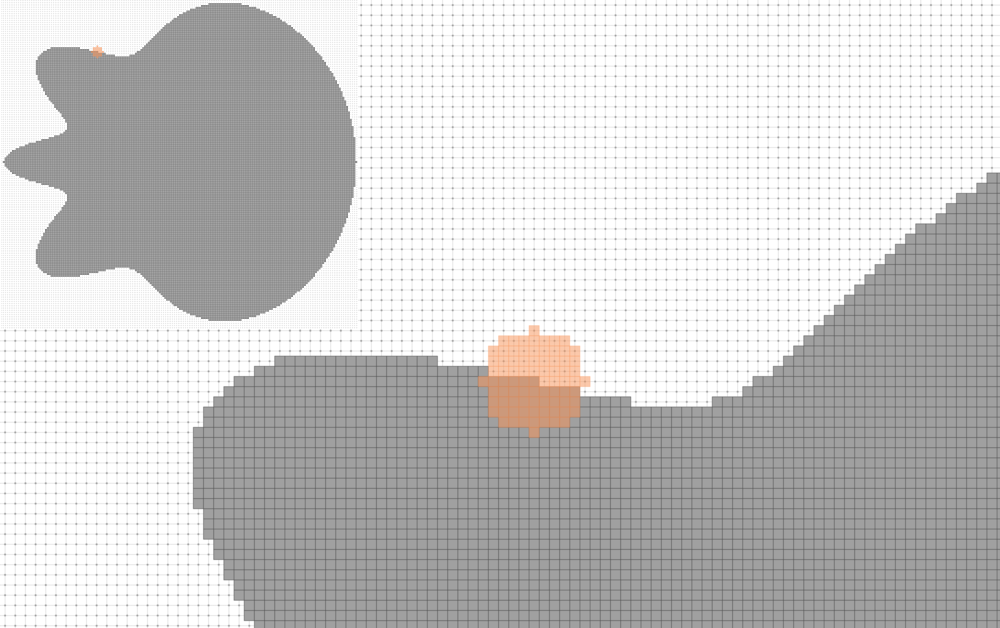
\includegraphics[scale=0.5]{figures/digital-estimators/ii/zoom/fr5-zoom.png}}%
		
	};
	\end{tikzpicture}	
	\end{figure}	
	}	

	\vspace{1.5em}

	\onslide<4->{
	\begin{align*}
		\hat{\kappa}(p) = \frac{3}{r^3}\left( \frac{\pi r^2}{2} - | B_r(p) \cap X | \right )
	\end{align*}}		
	
\end{frame}

\begin{frame}
	{Digital sets and convergent estimators}	
	{Conclusion}	

	\begin{itemize}
		\item{Digital sets are ambiguous and are constrained to the digital grid.}\\[1em]
		\item{The multigrid convergence is an adapted definition of convergence for geometric estimation on digital sets.}\\[2em]\pause
		\item[]{\textbf{Can we construct optimization models using multigrid convergent estimators?}}
	\end{itemize}

\end{frame}